\documentclass{standalone}
\usepackage{tikz,trees}
\begin{document}
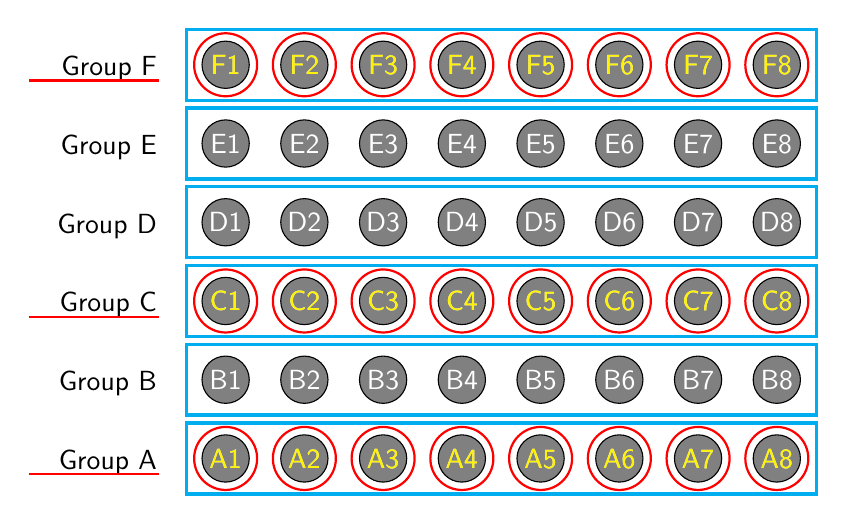
\begin{tikzpicture}[font=\sffamily]
	\edef\gnames{{"A","B","C","D","E","F"}};

	% Draw group backgrounds and labels (once per group)
	\foreach \grp in {1,2,...,6} {
	\pgfmathsetmacro\gname{\gnames[\grp-1]};
	\draw[cyan,very thick] (-0.5,{\grp-0.45}) rectangle (7.5,{\grp+0.45});
	\node[left] at (-0.75,{\grp-0.05}) {Group \gname};
	}

	% Draw all circles
	\foreach \grp in {1,2,...,6} {
		\pgfmathsetmacro\gname{\gnames[\grp-1]};
		\foreach \num in {1,2,...,8} {
			 \draw[fill=gray] ({\num-1},\grp) circle (0.3) node[white] (\num) {\gname\num};
			}
	}

	% Add red elements for specific groups
	\foreach \grp in {1,3,6} {
		\pgfmathsetmacro\gname{\gnames[\grp-1]};
		\draw[red,thick] (-2.5,{\grp-0.2}) -- (-0.85,{\grp-0.2});
		\foreach \num in {1,2,...,8} {
			 \draw[draw=red,thick] ({\num-1},\grp) circle (0.4) node[yellow] {\gname\num};
		}
	}
\end{tikzpicture}
\end{document}